\documentclass[convert = false, tikz]{standalone}
\usepackage[utf8]{inputenc}
\usepackage{tikz}
\usetikzlibrary{automata, positioning, arrows}
 
\usepackage{../../../../style_automata}

% arara: pdflatex
% arara: latexmk: { clean: partial }
\begin{document}
    \tikzset{
    node distance=2cm, % specifies the minimum distance between two nodes.
    }
    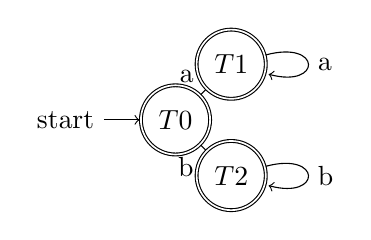
\begin{tikzpicture}
        \node[state, initial, accepting] (t0) {$T0$};
        \node[state, accepting, above right of=t0] (t1) {$T1$};
        \node[state, accepting, below right of=t0] (t2) {$T2$};
        \draw (t0) edge[above left] node{a} (t1)
        (t0) edge[below left] node{b} (t2)
        (t1) edge[loop right] node{a} (t1)
        (t2) edge[loop right] node{b} (t2);
    \end{tikzpicture}
\end{document}